\documentclass{article}

\usepackage{arxiv}

\usepackage[utf8]{inputenc} % allow utf-8 input
\usepackage[T1]{fontenc}    % use 8-bit T1 fonts
\usepackage{lmodern}        % https://github.com/rstudio/rticles/issues/343
\usepackage{hyperref}       % hyperlinks
\usepackage{url}            % simple URL typesetting
\usepackage{booktabs}       % professional-quality tables
\usepackage{amsfonts}       % blackboard math symbols
\usepackage{nicefrac}       % compact symbols for 1/2, etc.
\usepackage{microtype}      % microtypography
\usepackage{graphicx}

\title{The impact of accelerated COVID vaccine trials on mortality}

\author{
  }


% tightlist command for lists without linebreak
\providecommand{\tightlist}{%
  \setlength{\itemsep}{0pt}\setlength{\parskip}{0pt}}

% From pandoc table feature
\usepackage{longtable,booktabs,array}
\usepackage{calc} % for calculating minipage widths
% Correct order of tables after \paragraph or \subparagraph
\usepackage{etoolbox}
\makeatletter
\patchcmd\longtable{\par}{\if@noskipsec\mbox{}\fi\par}{}{}
\makeatother
% Allow footnotes in longtable head/foot
\IfFileExists{footnotehyper.sty}{\usepackage{footnotehyper}}{\usepackage{footnote}}
\makesavenoteenv{longtable}


\usepackage{natbib}
\begin{document}
\maketitle


\begin{abstract}

\end{abstract}


\hypertarget{abstract}{%
\section{Abstract}\label{abstract}}

\hypertarget{introduction}{%
\section{Introduction}\label{introduction}}

(this Introduction is copied from \href{https://docs.google.com/document/d/1YzVLaFWor03Y3jq8IBe2iXEhLd7PNW9srnLAerAXOfg/edit}{here}---for the time being please edit in Google Doc)
aa
The Covid-19 pandemic has had a devastating impact on global health and economies. In the United States and United Kingdom alone, hundreds of thousands of lives were lost in 2020 and 2021. The development and testing of vaccines for Covid-19 progressed at an unprecedented pace, with mass vaccinations beginning in some countries within less than a year from the start of the pandemic.

However, it has been suggested that the vaccines could have been made available even earlier. One proposal for acceleration has been the use of human challenge trials (HCTs) to test for efficacy. HCTs involve intentionally infecting a small group of volunteers with a disease in order to study the efficacy of potential treatments or vaccines. While both ethical and technological barriers to adoption of HCTs are considerable, they have the potential to significantly accelerate the efficacy studies.

In this paper, we aim to quantify the potential benefits of accelerating the approval and distribution of Covid-19 vaccines. While we focus on HCTs, the model we use is generic and applicable to all measures that could have led to earlier use of vaccines.

The potential benefits of accelerating the approval and distribution of vaccines, both in terms of health outcomes and economic impacts, are likely to be significant. In fact, research has suggested that these benefits may be orders of magnitude larger than the costs associated with acceleration (Castillo et al.~2021). Despite this, there has been relatively little research on the impact of speed on vaccination efforts, particularly in terms of epidemiological modeling.

A recent review paper (Więcek, 2022) found only one quantitative estimate of the impact of accelerating testing of vaccines on mortality. This estimate, from Berry et al.~(2020), was based on prospective simulations, which overestimated timelines for vaccine field trials and do not have information about the real burden of the Covid-19 pandemic in 2020 and 2021.

We use counterfactual simulations informed by retrospective analysis of data on observed vaccinations, infections, and mortality. This allows us to consider the actual vaccine development timelines. To quantify benefits of speed we consider different acceleration scenarios, estimate the number of vaccinations under each scenario, and then calculate the number of deaths averted, compared to the status quo.

We calculate benefits for two countries, the United States and the United Kingdom. They are large developed countries that were at the front of the queue for vaccine deliveries and therefore would have been likely to benefit from accelerated testing. It's good to contrast these two countries because they had epidemic waves occurring at different times, with different virus strains, and employed different non-pharmaceutical interventions.

Epidemiological modeling simplifies many nuances and may not consider certain factors, such as individual behaviors and responses to public health interventions. Therefore, we also include additional calculations, including both a theoretical model and a back-of-the-envelope calculation which ignores epidemiological spillovers. Additionally, we consider some potential unknowns associated with accelerating vaccine approvals, such as (1) less precise information on efficacy or safety, (2) impact on public confidence in vaccines, (3) the potential for production and distribution constraints to nullify the benefits of accelerated testing.

\hypertarget{methods}{%
\section{Methods}\label{methods}}

\hypertarget{baseline-model}{%
\subsection{Baseline model}\label{baseline-model}}

To model alternative vaccination timelines, we took an existing compartmental model that simulated the COVID-19 pandemic through 2020 and 2021 including the impact of vaccinations (the ``baseline model'') and re-ran the simulation freezing all parameters except the vaccination timelines (the ``counterfactual models'').

The baseline pandemic model used the model behind \citep{watsonoliverj.COVID19LMICReports2022}. This model is implemented in open source R packages Squire \citep[\citet{walkerImpactCOVID19Strategies2020}, \citet{watsonLeveragingCommunityMortality2021}]{hoganWithincountryAgebasedPrioritisation2021} and SirCOVID \citep{baguelinSircovidSIRModel2022}. An older version of this model is described in detail in the supplementary material of \citep{walkerImpactCOVID19Strategies2020}, and details of many parameters -- again, for an older version of the model -- can be found in the supplementary material of \citep{watsonGlobalImpactFirst2022}. Additional incomplete information about the parametrisation of the version of the model we used can be found at \href{https://web.archive.org/web/20221230232942/https://mrc-ide.github.io/global-lmic-reports/parameters.html}{COVID-19 LMIC Reports documentation} \citep{watsonoliverj.COVID19LMICReports2022}, and more up-to-date but less complete model structure can be found in the \href{https://web.archive.org/web/20221230232915/https://mrc-ide.github.io/nimue/index.html}{Nimue documentation} \citep{winskillNimue}. Here we will describe the model in broad terms.

The baseline model is an age-stratified SEIRD model. In addition to classifying the population by infection status, the model also classifies people by vaccination status: they may be unvaccinated, vaccinated with 1 dose, vaccinated with 2 doses, vaccinated with 2 doses with waned protection, vaccinated 3 doses and vaccinated with 3 doses with waned protection. People are vaccinated according to vaccination dosage data from Our World in Data \citep{mathieuCoronavirusPandemicCOVID192020} together with a model of vaccine prioritisation. They progress to ``waned'' classes according to an assumed rate of waning of vaccine-derived immunity, which is itself time and dose-number-dependent. The model accounts for separate modes of vaccine action (infection blocking vs disease blocking), variant-dependent efficacy of vaccine and naturally derived immunity and age-dependent vaccination strategies.

The model assumes homogenous mixing of the population. It models different kinds of infection -- ``severe'' and ``non-severe'' -- which have different age-dependent probabilities of progressing to recovery or death. Individuals who have recovered are assumed to be fully protected by natural immunity for an exponentially random duration duration which is, on average, around 250 days. Individuals who have been vaccinated have different levels of protection at different points in time depending on the dominant strain, and unless they receive additional doeses then protection is considered to have waned after an exponentially random period of time (on average, around 150 days). Vaccinated individuals are also considered to have a reduced likelihood of onward transmission, which also fades when the vaccine protection wanes.

The model features a mix of deterministic parameters and random parameters. We run an ensemble of simulations for each country, sampling the random parameters at the start of each run from pre-defined distributions. The initial number of cases seeding the pandemic in the country and the time series of reproduction numbers of infections in a fully susceptible population \(R_t\) is then fit to the observed course of deaths during the time period associated with the simulation.

The distributions of random parameters is given in Table \ref{tab:trajectory-sampling-parameters}. Parameters are sampled from each distribution independently except for the duration of vaccine-derived immunity, which is dependent on vaccine efficacy. 100 sets of parameters are sampled, and epidemic trajectories simulated for each. 95\% intervals in our results refer to percentiles among the set of 100 sampled trajectories, so a 95\% interval for deaths averted is the pair of numbers given by the 2.5th and the 97.5th percentile of deaths averted among all sampled trajectories. Note that the distributions given here are not exact representations of the models sampling distributions, which involve additional truncation steps.

The model of \citep{watsonoliverj.COVID19LMICReports2022} also samples probabilities of hospitalisation and mechanical ventilation for each trajectory, but these play no role in our analysis not already captured by the infection fatality rate, and so we haven't reported on the relevant parameters here.

The shape parameters \(\alpha_e^P, \beta_e^P\) that appear in Table \ref{tab:trajectory-sampling-parameters} are the shape parameters associated with a beta distribution with mean \(\mu_e^P\) and variance \(0.005\). The mean \(\mu_e^P\) is determined by estimating the efficacy of each vaccine platform \(P\) against each variant (see Table \ref{tab:vaccine-efficacy}). The mean vaccine durations are determined according to models of antibody decay, and are dependent on the sampled vaccine efficacies \(\mu_e^P\) \citep{watsonoliverj.COVID19LMICReports2022}.

\begin{table}

\caption{\label{tab:trajectory-sampling-parameters}Distributions from which parameters are sampled. The parameters $\alpha_e^P, \beta_e^P$ are shape parameters for vaccine platform $P$ with associated dominant strain dependent efficacy $e$ (see text for additional details). The parameters $\alpha_d, \beta_d$ are shape and rate parameters for distribution of vaccine durations, determined by fitting an antibody decay curve to vaccine efficacies. $\mathrm{rescale}(\cdot, f_{min}, f_{med}, f_{max})$ is a function that maps $0$ to $f_{min}$, $0.5$ to $f_{med}$ and $1$ to $f_{max}$, linearly interpolating between each. $f_{min}, f_{med}, f_{max}$ are respectively the minimum, median, and maximum estimates of age-adjusted infection fatality.}
\centering
\begin{tabular}[t]{ll}
\toprule
Parameter & Distribution\\
\midrule
Vaccine efficacy $V$ & $V\sim \mathrm{Beta}(\alpha_{e}^P, \beta_{e}^P), P\sim U(\{\mathrm{vaccine platforms}\})$\\
Vaccine duration $D$ & $\frac{1}{\mathrm{Gamma}(\alpha_{d}, \beta_d)}$\\
Infection fatality rate with treatment $F$ & $F = \mathrm{rescale}(X,f_{min}, f_{med}, f_{max})\quad X\sim \mathrm{Beta}(2,2)$\\
\bottomrule
\end{tabular}
\end{table}

\begin{table}

\caption{\label{tab:vaccine-platforms}Vaccine platforms used by each country.}
\centering
\begin{tabular}[t]{ll}
\toprule
Country & Platforms\\
\midrule
USA & mRNA, single dose, subunit\\
UK & adenovirus, mRNA\\
\bottomrule
\end{tabular}
\end{table}

\begin{table}

\caption{\label{tab:vaccine-efficacy}Model parameters - central estimates of vaccine efficacy}
\centering
\begin{tabular}[t]{lllr}
\toprule
Vaccine type & Doses & Strain & Protection against infection\\
\midrule
mRNA & 1 & Wild & 0.630\\
mRNA & 2 & Wild & 0.860\\
mRNA & 1 & Delta & 0.360\\
mRNA & 2 & Delta & 0.880\\
mRNA & 1 & Omicron & 0.000\\
mRNA & 2 & Omicron & 0.136\\
mRNA & 3 & Omicron & 0.650\\
Single dose & Full & Wild & 0.660\\
Single dose & Full & Delta & 0.500\\
Adenovirus & Partial & Wild & 0.640\\
Adenovirus & Full & Wild & 0.770\\
Adenovirus & Partial & Delta & 0.300\\
Adenovirus & Full & Delta & 0.670\\
Subunit & Partial & Wild & 0.540\\
Subunit & Full & Wild & 0.860\\
Subunit & Partial & Delta & 0.300\\
Subunit & Full & Delta & 0.710\\
\bottomrule
\end{tabular}
\end{table}

We made one change to the model used by \citep{watsonoliverj.COVID19LMICReports2022}: by default, vaccination was assumed to reduce onward transmission by 50\%, regardless of whether the dose was fresh or waned. We modified this to the schedule shown in Table \ref{tab:onward}. These represented an average between the estimates of \citep{eyreImpactSARSCoV2Vaccination2021a} for effectiveness at blocking onward transmission of Alpha and Delta and the estimate of \citep{tanInfectiousnessSARSCoV2Breakthrough2023} for effectiveness of the vaccine at blocking onward transmission of Omicron, as the period of the simulation included both Delta and Omicron waves.

\begin{table}

\caption{\label{tab:onward}Assumed relative transmissibility of infection by vaccinated individuals compared to unvaccinated}
\centering
\begin{tabular}[t]{ll}
\toprule
Doses & Protection from onward transmission\\
\midrule
1 dose (fresh) & 27\%\\
2 doses (fresh) & 27\%\\
2 doses (waned) & 0\%\\
3 doses (fresh) & 30\%\\
3 doses (waned stage 1) & 10\%\\
3 doses (waned stage 2) & 5\%\\
\bottomrule
\end{tabular}
\end{table}

\hypertarget{vaccine-production}{%
\subsection{Vaccine production}\label{vaccine-production}}

To produce counterfactual vaccine dosage timeseries, we suppose that vaccine approcal is brought forward by a number of days (we test approval coming 30, 60 and 90 day sooner). However, if approval is brought forward too much then manufacturers might have a harder time maintaining supply than they would have in the situation that actually played out. We model this by \ldots{} (see Tomas' entry in the shared doc)

Plots can currently be found in \protect\hyperlink{vaccine-production-model}{Vaccine production model}

\hypertarget{results}{%
\section{Results}\label{results}}

\hypertarget{vaccinations-under-counterfactual-scenarios}{%
\subsection{Vaccinations under counterfactual scenarios}\label{vaccinations-under-counterfactual-scenarios}}

Figure \ref{fig:cumul-vacc-cfacts} shows the cumulative vaccinations for the counterfactual scenarios we investigate. The baseline scenario is the actual vaccination timeline, while the other scenarios are the same timeline but with vaccines administered 30, 60 or 90 days sooner.

\begin{figure}

{\centering 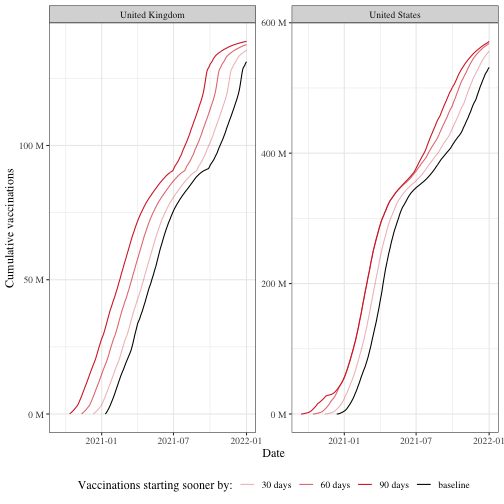
\includegraphics{_main_files/figure-latex/cumul-vacc-cfacts-1} 

}

\caption{DJ4 Cumulative vaccine counterfactuals}\label{fig:cumul-vacc-cfacts}
\end{figure}

Table \ref{tab:vaccinations-table} shows the actual vaccinations administered on 2021-01-01, 2021-04-01 and 2021-07-01 alongside the administration numbers for the counterfactual scenarios we investigage.

\begin{verbatim}
## The following `from` values were not present in `x`: Counterfactual scenario
\end{verbatim}

\begin{table}

\caption{\label{tab:vaccinations-table}Total vaccinations at sample dates}
\centering
\begin{tabular}[t]{llll}
\toprule
shifted\_by & 2021-01-01 & 2021-04-01 & 2021-07-01\\
\midrule
\addlinespace[0.3em]
\multicolumn{4}{l}{\textbf{United Kingdom}}\\
\hspace{1em}Baseline & 0 & 33,337,926 & 75,688,766\\
\hspace{1em}Vaccines 30 days sooner & 3,460,361 & 42,486,427 & 80,736,395\\
\hspace{1em}Vaccines 60 days sooner & 14,859,054 & 57,449,853 & 86,771,215\\
\hspace{1em}Vaccines 90 days sooner & 28,042,344 & 71,663,088 & 91,140,069\\
\addlinespace[0.3em]
\multicolumn{4}{l}{\textbf{United States}}\\
\hspace{1em}Baseline & 4,521,988 & 172,124,225 & 347,123,032\\
\hspace{1em}Vaccines 30 days sooner & 23,889,241 & 238,670,399 & 357,876,350\\
\hspace{1em}Vaccines 60 days sooner & 56,107,462 & 289,245,438 & 372,702,522\\
\hspace{1em}Vaccines 90 days sooner & 56,107,489 & 289,245,510 & 376,955,754\\
\bottomrule
\end{tabular}
\end{table}

\hypertarget{impact-of-counterfactual-vaccination-scenarios}{%
\subsection{Impact of counterfactual vaccination scenarios}\label{impact-of-counterfactual-vaccination-scenarios}}

Table \ref{tab:deaths-averted-table} shows the number of deaths averted by each counterfactual scenario. The number of deaths averted is calculated as the difference between the number of deaths under the baseline scenario and the number of deaths under the counterfactual scenario. The number of deaths averted is shown as the average number of deaths averted, as well as the interval that contains 95\% of simulation trajectories (see Section \protect\hyperlink{methods}{Methods} for details on how simulation trajectories are sampled). The number of deaths averted is also shown as the average number of deaths averted per 10,000 people in each country.

\begin{verbatim}
## Warning: Using `all_of()` outside of a selecting function was deprecated in tidyselect 1.2.0.
## i See details at <https://tidyselect.r-lib.org/reference/faq-selection-context.html>
## This warning is displayed once every 8 hours.
## Call `lifecycle::last_lifecycle_warnings()` to see where this warning was generated.
\end{verbatim}

\begin{verbatim}
## The following `from` values were not present in `x`: Counterfactual scenario, Deaths averted, Deaths averted per 10,000, Baseline deaths, Deaths averted per baseline death
\end{verbatim}

\begin{table}

\caption{\label{tab:deaths-averted-table}DJ5 Averted deaths}
\centering
\fontsize{7}{9}\selectfont
\begin{tabular}[t]{lllrr}
\toprule
counterfactual\_label & delta\_deaths & delta\_deaths\_perpop & baseline\_cumulative\_deaths\_avg & delta\_deaths\_perreported\\
\midrule
\addlinespace[0.3em]
\multicolumn{5}{l}{\textbf{United Kingdom to April 2021}}\\
\hspace{1em}30 days sooner & 5,682 [4,250; 9,361] & 0.85 [0.63; 1.40] & 140486 & 0.04\\
\hspace{1em}60 days sooner & 16,024 [13,351; 25,544] & 2.39 [1.99; 3.81] & 140486 & 0.11\\
\hspace{1em}90 days sooner & 26,942 [23,165; 35,453] & 4.02 [3.45; 5.29] & 140486 & 0.19\\
\addlinespace[0.3em]
\multicolumn{5}{l}{\textbf{United Kingdom to July 2021}}\\
\hspace{1em}30 days sooner & 5,959 [4,655; 9,242] & 0.89 [0.69; 1.38] & 143115 & 0.04\\
\hspace{1em}60 days sooner & 17,900 [14,991; 26,488] & 2.67 [2.23; 3.95] & 143115 & 0.13\\
\hspace{1em}90 days sooner & 29,616 [25,497; 36,711] & 4.41 [3.80; 5.47] & 143115 & 0.21\\
\addlinespace[0.3em]
\multicolumn{5}{l}{\textbf{United Kingdom to Jan 2022}}\\
\hspace{1em}30 days sooner & 10,290 [8,657; 14,397] & 1.53 [1.29; 2.15] & 174302 & 0.06\\
\hspace{1em}60 days sooner & 38,221 [32,957; 41,018] & 5.70 [4.91; 6.11] & 174302 & 0.22\\
\hspace{1em}90 days sooner & 56,926 [51,235; 59,932] & 8.49 [7.64; 8.93] & 174302 & 0.33\\
\addlinespace[0.3em]
\multicolumn{5}{l}{\textbf{United States to April 2021}}\\
\hspace{1em}30 days sooner & 17,343 [2,871; 37,637] & 0.52 [0.09; 1.14] & 643041 & 0.03\\
\hspace{1em}60 days sooner & 54,609 [13,318; 104,973] & 1.65 [0.40; 3.17] & 643041 & 0.08\\
\hspace{1em}90 days sooner & 78,091 [29,336; 138,458] & 2.36 [0.88; 4.18] & 643041 & 0.12\\
\addlinespace[0.3em]
\multicolumn{5}{l}{\textbf{United States to July 2021}}\\
\hspace{1em}30 days sooner & 33,093 [12,630; 48,999] & 1.00 [0.38; 1.48] & 684646 & 0.05\\
\hspace{1em}60 days sooner & 80,747 [32,170; 122,491] & 2.44 [0.97; 3.70] & 684646 & 0.12\\
\hspace{1em}90 days sooner & 102,180 [47,565; 150,268] & 3.08 [1.43; 4.53] & 684646 & 0.15\\
\addlinespace[0.3em]
\multicolumn{5}{l}{\textbf{United States to Jan 2022}}\\
\hspace{1em}30 days sooner & 57,879 [-34,415; 126,631] & 1.75 [-1.04; 3.82] & 978291 & 0.06\\
\hspace{1em}60 days sooner & 153,618 [-30,648; 258,929] & 4.63 [-0.92; 7.81] & 978291 & 0.16\\
\hspace{1em}90 days sooner & 240,451 [96,025; 311,001] & 7.25 [2.90; 9.38] & 978291 & 0.25\\
\bottomrule
\end{tabular}
\end{table}

Figure \ref{fig:deaths-averted-plot} shows the number of deaths per day under each counterfactual scenario compared to the baseline. Also shown is the interval containing 95\% of the counterfactual simulation trajectories. Figure @ref\{cumulative-deaths\} shows cumulative deaths under the baseline and counterfactual scenarios.

\begin{figure}

{\centering 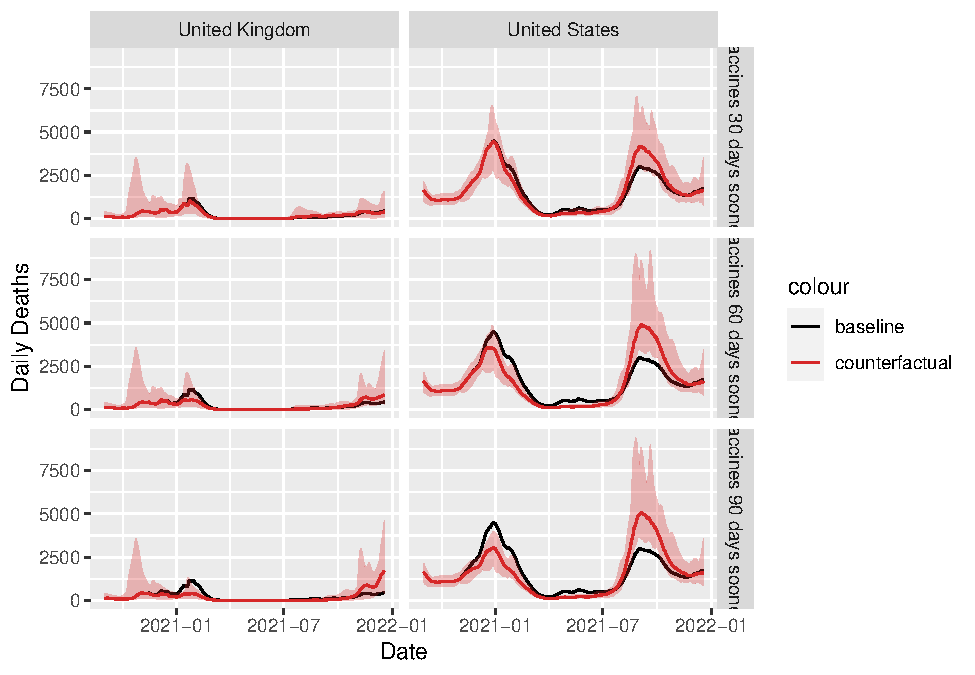
\includegraphics{_main_files/figure-latex/deaths-averted-plot-1} 

}

\caption{DJ6 Daily deaths per scenario}\label{fig:deaths-averted-plot}
\end{figure}

\begin{figure}

{\centering 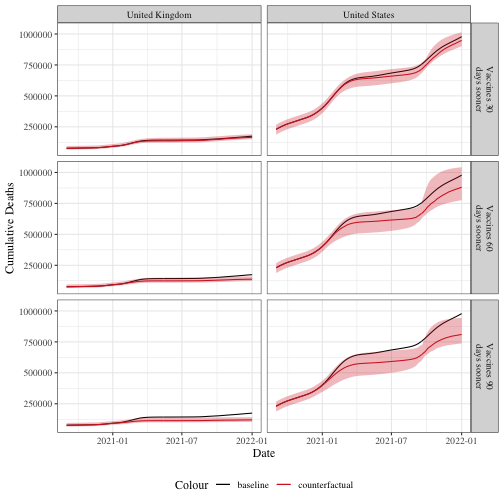
\includegraphics{_main_files/figure-latex/cumulative-deaths-1} 

}

\caption{Cumulative deaths per scenario}\label{fig:cumulative-deaths}
\end{figure}

\hypertarget{discussion}{%
\section{Discussion}\label{discussion}}

\hypertarget{placeholder-for-commentary-on-main-results}{%
\subsection{Placeholder for commentary on main results}\label{placeholder-for-commentary-on-main-results}}

\hypertarget{subsequent-infection-waves}{%
\subsection{Subsequent infection waves}\label{subsequent-infection-waves}}

While our main results present the number of deaths averted up to July 2021, we simulated the counterfactual scenarious up until the end of 2021. The longer timeline includes an additional wave of infections in both the US and the UK. Our model shows much more uncertainty over the effect of earlier vaccination timelines for this second wave of infections in the United States. In this country, the 95\% interval of simulation traces ranges from 228 000 lives saved to 90 000 extra deaths. The UK, on the other hand, shows much less variation in the impact of earlier timelines on the number of deaths in the second wave.

There are numerous ways that altering the timing of vaccinations can alter the pandemic trajectory for subsequent waves of infection. Effects that enter into our model are:
1. Earlier vaccine administration means that people will experience waning vaccine protection earlier, which could make them vulnerable if this waning coincides with a peak in infections (this is expected to increase infections at later dates)
2. Earlier vaccine administration can reduce the total number of infections immediately following the vaccination campaign, leading to fewer people having naturally acquired immunity at later dates (this is expected to increase infections at later dates)
3. Earlier vaccine administration can reduce the number of people infected at the start of a followup wave of infections (this is expected to increase the time taken to reach an infection peak and reduce the overall number of infections)
4. Earlier vaccine administration goes together with earlier administration of booster doses, so people may be \emph{more} protected at followup waves due to having recently received a booster (this is expected to reduce the overall number of infections)

Earlier vaccine administration may also lead to behaviour change, which is not captured by our model. The effect of behaviour change downstream of vaccination is also hard to predict. If earlier vaccination leads to fewer infections in deaths at a given point in time, and as a result people relax social distancing behaviour, then our model might overestimate short-term infections and deaths in the early vaccination scenario (though people would of course be benefiting from reduced social distancing). At the same time, such a situation would lead to a higher rate of natural immunity, which could reduce the impact of a subsequent infection wave.

We hypothesise that differences between the US and the UK that lead to the divergent results may be:
- Booster doses were much more popular in the UK than in the US. On Jan 1 2022 50.5\% of the UK population had received booster doses compared to 23.4\% of the US population \citep{mathieuCoronavirusPandemicCOVID192020}
- Our model predicts that in the short run, earlier vaccinations suppress the level of infections in the UK more than they do in the US.

To test the hypothesis that differential booster doses explain some of the difference, we ran a simulation where the rate of booster doses in the US was counterfactually adjusted so that the coverage of booster doses in both the US and UK were equal on Jan 1 2022 (to achieve this, we rougly doubled the booster dose coverage in the US). The results are in Supplementary Table \ref{tab:deaths-averted-table-doubleboost}. We note that this counterfactual doesn't drastically reduce the uncertainty over long run deaths averted in the US, suggesting that the differences between the US and the UK estimates are driven by something other than differences in booster adoption.

While we show that earlier vaccinations have large benefits to mortality in infections waves occurring close to the vaccination campaign, and our best guess is that earlier vaccinations yield large benefits to mortality overall, we are substantially less certain of the latter conclusion. Due to uncertainty about the effects of early vaccination on followup waves, we are substantially uncertain about the overall size and sign of the mortality benefit for COVID-19. Furthermore, future pandemics (or even followup waves of COVID-19) are going to differ from the period we studied, and the overall benefits of accelerated vaccinations are likely to be sensitive to these differences.

\hypertarget{sensitivity-to-modelling-assumptions}{%
\subsection{Sensitivity to modelling assumptions}\label{sensitivity-to-modelling-assumptions}}

We explored various alternative model configurations in order to assess the sensitivity of our conclusion to modelling assumptions. Compared to a hypothetical ideal model that yields correct counterfactual assessments, the model we employ is likely to differ in a number of ways:
- It may differ structurally. We might anticipate some structural differences - for example, overdispersion in the distribution of contact rates is not captured by our model, but overdispersion in this distribution was typically found to be high \citep{endoEstimatingOverdispersionCOVID192020}. However, there may be other structural differences that we do not anticipate
- The assumed distributions of input parameters may differ in our model and in the hypothetical ideal

Both of these differences mean that the fitted values of \(R_t\) are also likely to differ between our model and the hypothetical ideal, and hence they may yield substantially different assessments of counterfactual scenarios. If it turns out that counterfactual assessments are very sensitive to input parameter values, then we might conclude that our estimates are likely to differ substantially from the ``true'' counterfactual. Because of the prospect of structural differences, this is true even if we have done a very good job of estimating parameters. If our results are robust to variation of parameters within a reasonable range, then if we believe that our model is capable of yielding a good approximation to the ideal for some ``reaonsable'' parameter choices, we should also think our counterfactual assessments are a good approximation to ideal counterfactual assessments.

We assess the impact of three different parameter estimates on our overall results. To do this, we examine the average conclusion from the model runs featuring the top and bottom deciles of each of the following parameters:
- The average infection-blocking efficacy of one and two doses of the vaccine
- The average duration for protection due to one and two doses of the vaccine
- The average duration of protection due to natural immunity

In both countries, the estimates of deaths averted showed little sensitivity to the estimated duration of natural immunity (Supplementary Table \ref{tab:deaths-averted-table-durR}. The estimates of deaths averted in the UK was \emph{also} relatively insensitive to the estimated vaccine efficacy, though the estimate in the US was more sensitive to this value (it is worth noting that in the case of the US the model explored captured a wider range of variation in vaccine efficacy) - see Supplementary Table \ref{tab:deaths-averted-table-vei}. Note that for long-run estimates of deaths averted in the US (up to Jan 2022), higher estimates of vaccine efficacy were associated with much greater uncertainty over the number of deaths averted. This may be due to the fact that, given a more effective vaccine, waning immunity will have a larger impact on the end results.

The estimate of long-run deaths averted in the US was extremely sensitive to the estimated duration of vaccine derived immunity, with a difference of 14 days in this parameter estimate yielding long-run estimates of deaths averted that ranged from 32 255 to \emph{negative} 11 456 (that is, 11 456 extra deaths) for a 30 day advance in the vaccination schedule. Notably, short estimates of vaccine duration were also associated with extreme decreases in the uncertainty over the number of deaths averted. Note that the short run estimates of deaths averted (up to July 2021) were robustly positive, but were also substantially more uncertain for longer estimates of the duration of vaccine protection.

Our model is already very uncertain about the effect of earlier vaccinations on the second infection wave in the US. However, the high sensitivity of this figure to the estimated duration of vaccine-derived protection offers an extra reason to be unsure that the model is providing us with an accurate assessment of the counterfactual impacts on this timescale.

We also run an identical analysis to our main analysis, except with a model fit to reported numbers of COVID-19 deaths instead of COVID-19 deaths estimated from excess mortality. The results are reported in Supplementary Table \ref{tab:reported-deaths-averted-table} and Supplementary Figure \ref{fig:reported-deaths-averted-plot}. This method yields larger estimates of deaths averted than our main method, particularly up to July 2021 where the estimates are close to the 95th percentile estimate for the main method. This is in spite of the fact that the total estimated number of deaths under this method is somewhat lower than under the excess mortality method.

\hypertarget{conclusion}{%
\section{Conclusion}\label{conclusion}}

\bibliography{report.bib}

\hypertarget{appendix-appendix}{%
\appendix}


\hypertarget{sensitivity}{%
\section{Sensitivity}\label{sensitivity}}

\hypertarget{baseline-fit-to-reported-deaths-instead-of-excess-deaths}{%
\subsection{Baseline fit to reported deaths instead of excess deaths}\label{baseline-fit-to-reported-deaths-instead-of-excess-deaths}}

\begin{verbatim}
## The following `from` values were not present in `x`: Counterfactual scenario, Deaths averted, Deaths averted per 10,000, Baseline deaths, Deaths averted per baseline death
\end{verbatim}

\begin{table}

\caption{\label{tab:reported-deaths-averted-table}Averted deaths calculated on the basis of a model fit to reported deaths}
\centering
\fontsize{7}{9}\selectfont
\begin{tabular}[t]{lllrr}
\toprule
counterfactual\_label & delta\_deaths & delta\_deaths\_perpop & baseline\_cumulative\_deaths\_avg & delta\_deaths\_perreported\\
\midrule
\addlinespace[0.3em]
\multicolumn{5}{l}{\textbf{United Kingdom to April 2021}}\\
\hspace{1em}30 days sooner & 5,682 [4,250; 9,361] & 0.85 [0.63; 1.40] & 140486 & 0.04\\
\hspace{1em}60 days sooner & 16,024 [13,351; 25,544] & 2.39 [1.99; 3.81] & 140486 & 0.11\\
\hspace{1em}90 days sooner & 26,942 [23,165; 35,453] & 4.02 [3.45; 5.29] & 140486 & 0.19\\
\addlinespace[0.3em]
\multicolumn{5}{l}{\textbf{United Kingdom to July 2021}}\\
\hspace{1em}30 days sooner & 5,959 [4,655; 9,242] & 0.89 [0.69; 1.38] & 143115 & 0.04\\
\hspace{1em}60 days sooner & 17,900 [14,991; 26,488] & 2.67 [2.23; 3.95] & 143115 & 0.13\\
\hspace{1em}90 days sooner & 29,616 [25,497; 36,711] & 4.41 [3.80; 5.47] & 143115 & 0.21\\
\addlinespace[0.3em]
\multicolumn{5}{l}{\textbf{United Kingdom to Jan 2022}}\\
\hspace{1em}30 days sooner & 10,290 [8,657; 14,397] & 1.53 [1.29; 2.15] & 174302 & 0.06\\
\hspace{1em}60 days sooner & 38,221 [32,957; 41,018] & 5.70 [4.91; 6.11] & 174302 & 0.22\\
\hspace{1em}90 days sooner & 56,926 [51,235; 59,932] & 8.49 [7.64; 8.93] & 174302 & 0.33\\
\addlinespace[0.3em]
\multicolumn{5}{l}{\textbf{United States to April 2021}}\\
\hspace{1em}30 days sooner & 17,343 [2,871; 37,637] & 0.52 [0.09; 1.14] & 643041 & 0.03\\
\hspace{1em}60 days sooner & 54,609 [13,318; 104,973] & 1.65 [0.40; 3.17] & 643041 & 0.08\\
\hspace{1em}90 days sooner & 78,091 [29,336; 138,458] & 2.36 [0.88; 4.18] & 643041 & 0.12\\
\addlinespace[0.3em]
\multicolumn{5}{l}{\textbf{United States to July 2021}}\\
\hspace{1em}30 days sooner & 33,093 [12,630; 48,999] & 1.00 [0.38; 1.48] & 684646 & 0.05\\
\hspace{1em}60 days sooner & 80,747 [32,170; 122,491] & 2.44 [0.97; 3.70] & 684646 & 0.12\\
\hspace{1em}90 days sooner & 102,180 [47,565; 150,268] & 3.08 [1.43; 4.53] & 684646 & 0.15\\
\addlinespace[0.3em]
\multicolumn{5}{l}{\textbf{United States to Jan 2022}}\\
\hspace{1em}30 days sooner & 57,879 [-34,415; 126,631] & 1.75 [-1.04; 3.82] & 978291 & 0.06\\
\hspace{1em}60 days sooner & 153,618 [-30,648; 258,929] & 4.63 [-0.92; 7.81] & 978291 & 0.16\\
\hspace{1em}90 days sooner & 240,451 [96,025; 311,001] & 7.25 [2.90; 9.38] & 978291 & 0.25\\
\bottomrule
\end{tabular}
\end{table}

\begin{figure}

{\centering \includegraphics{_main_files/figure-latex/reported-deaths-averted-plot-1} 

}

\caption{DJ6 Daily deaths per scenario}\label{fig:reported-deaths-averted-plot}
\end{figure}

\hypertarget{counterfactual-scenario-what-if-us-had-doubled-the-rate-of-booster-uptake}{%
\subsection{Counterfactual scenario: what if US had doubled the rate of booster uptake?}\label{counterfactual-scenario-what-if-us-had-doubled-the-rate-of-booster-uptake}}

\begin{verbatim}
## The following `from` values were not present in `x`: Counterfactual scenario, Deaths averted, Deaths averted per 10,000, Baseline deaths, Deaths averted per baseline death
\end{verbatim}

\begin{table}

\caption{\label{tab:deaths-averted-table-doubleboost}How would US outcomes change if boosters were adopted at twice the actual rate?}
\centering
\fontsize{7}{9}\selectfont
\begin{tabular}[t]{lllrr}
\toprule
counterfactual\_label & delta\_deaths & delta\_deaths\_perpop & baseline\_cumulative\_deaths\_avg & delta\_deaths\_perreported\\
\midrule
\addlinespace[0.3em]
\multicolumn{5}{l}{\textbf{United Kingdom to April 2021}}\\
\hspace{1em}30 days sooner & 5,682 [4,250; 9,361] & 0.85 [0.63; 1.40] & 140486 & 0.04\\
\hspace{1em}60 days sooner & 16,024 [13,351; 25,544] & 2.39 [1.99; 3.81] & 140486 & 0.11\\
\hspace{1em}90 days sooner & 26,942 [23,165; 35,453] & 4.02 [3.45; 5.29] & 140486 & 0.19\\
\addlinespace[0.3em]
\multicolumn{5}{l}{\textbf{United Kingdom to July 2021}}\\
\hspace{1em}30 days sooner & 5,959 [4,655; 9,242] & 0.89 [0.69; 1.38] & 143115 & 0.04\\
\hspace{1em}60 days sooner & 17,900 [14,991; 26,488] & 2.67 [2.23; 3.95] & 143115 & 0.13\\
\hspace{1em}90 days sooner & 29,616 [25,497; 36,711] & 4.41 [3.80; 5.47] & 143115 & 0.21\\
\addlinespace[0.3em]
\multicolumn{5}{l}{\textbf{United Kingdom to Jan 2022}}\\
\hspace{1em}30 days sooner & 10,290 [8,657; 14,397] & 1.53 [1.29; 2.15] & 174302 & 0.06\\
\hspace{1em}60 days sooner & 38,221 [32,957; 41,018] & 5.70 [4.91; 6.11] & 174302 & 0.22\\
\hspace{1em}90 days sooner & 56,926 [51,235; 59,932] & 8.49 [7.64; 8.93] & 174302 & 0.33\\
\addlinespace[0.3em]
\multicolumn{5}{l}{\textbf{United States to April 2021}}\\
\hspace{1em}30 days sooner & 17,343 [2,871; 37,637] & 0.52 [0.09; 1.14] & 643041 & 0.03\\
\hspace{1em}60 days sooner & 54,609 [13,318; 104,973] & 1.65 [0.40; 3.17] & 643041 & 0.08\\
\hspace{1em}90 days sooner & 78,091 [29,336; 138,458] & 2.36 [0.88; 4.18] & 643041 & 0.12\\
\addlinespace[0.3em]
\multicolumn{5}{l}{\textbf{United States to July 2021}}\\
\hspace{1em}30 days sooner & 33,093 [12,630; 48,999] & 1.00 [0.38; 1.48] & 684646 & 0.05\\
\hspace{1em}60 days sooner & 80,747 [32,170; 122,491] & 2.44 [0.97; 3.70] & 684646 & 0.12\\
\hspace{1em}90 days sooner & 102,180 [47,565; 150,268] & 3.08 [1.43; 4.53] & 684646 & 0.15\\
\addlinespace[0.3em]
\multicolumn{5}{l}{\textbf{United States to Jan 2022}}\\
\hspace{1em}30 days sooner & 57,879 [-34,415; 126,631] & 1.75 [-1.04; 3.82] & 978291 & 0.06\\
\hspace{1em}60 days sooner & 153,618 [-30,648; 258,929] & 4.63 [-0.92; 7.81] & 978291 & 0.16\\
\hspace{1em}90 days sooner & 240,451 [96,025; 311,001] & 7.25 [2.90; 9.38] & 978291 & 0.25\\
\bottomrule
\end{tabular}
\end{table}

\hypertarget{sensitivity-to-parametric-estimates}{%
\subsection{Sensitivity to parametric estimates}\label{sensitivity-to-parametric-estimates}}

\begin{verbatim}
## The following `from` values were not present in `x`: Counterfactual scenario, Deaths averted, sensitivity_value, Deaths averted per 10,000, Baseline deaths, Averted/baseline
## The following `from` values were not present in `x`: Counterfactual scenario, Deaths averted, sensitivity_value, Deaths averted per 10,000, Baseline deaths, Averted/baseline
## The following `from` values were not present in `x`: Counterfactual scenario, Deaths averted, sensitivity_value, Deaths averted per 10,000, Baseline deaths, Averted/baseline
\end{verbatim}

\begin{table}

\caption{\label{tab:deaths-averted-table-vei}Sensitivity to average vaccine efficacy against infection (VEI)}
\centering
\fontsize{7}{9}\selectfont
\begin{tabular}[t]{lrllrr}
\toprule
counterfactual\_label & sensitivity\_value\_avg & delta\_deaths & delta\_deaths\_perpop & baseline\_cumulative\_deaths\_avg & delta\_deaths\_perreported\\
\midrule
\addlinespace[0.3em]
\multicolumn{6}{l}{\textbf{UK to April 2021}}\\
\hspace{1em}30 days sooner & 0.27 & 5,427 [4,730; 6,421] & 0.81 [0.71; 0.96] & 138248 & 0.04\\
\hspace{1em}30 days sooner & 0.47 & 6,373 [5,240; 7,244] & 0.95 [0.78; 1.08] & 133936 & 0.05\\
\hspace{1em}60 days sooner & 0.27 & 15,387 [14,162; 17,731] & 2.29 [2.11; 2.64] & 138248 & 0.11\\
\hspace{1em}60 days sooner & 0.47 & 17,665 [15,618; 19,046] & 2.63 [2.33; 2.84] & 133936 & 0.13\\
\hspace{1em}90 days sooner & 0.27 & 25,371 [24,364; 28,164] & 3.78 [3.63; 4.20] & 138248 & 0.18\\
\hspace{1em}90 days sooner & 0.47 & 28,046 [26,325; 29,582] & 4.18 [3.92; 4.41] & 133936 & 0.21\\
\addlinespace[0.3em]
\multicolumn{6}{l}{\textbf{UK to July 2021}}\\
\hspace{1em}30 days sooner & 0.27 & 5,734 [5,058; 6,640] & 0.85 [0.75; 0.99] & 140544 & 0.04\\
\hspace{1em}30 days sooner & 0.47 & 6,620 [5,575; 7,497] & 0.99 [0.83; 1.12] & 136056 & 0.05\\
\hspace{1em}60 days sooner & 0.27 & 17,066 [15,874; 18,665] & 2.54 [2.37; 2.78] & 140544 & 0.12\\
\hspace{1em}60 days sooner & 0.47 & 18,706 [17,287; 20,048] & 2.79 [2.58; 2.99] & 136056 & 0.14\\
\hspace{1em}90 days sooner & 0.27 & 28,057 [26,771; 29,984] & 4.18 [3.99; 4.47] & 140544 & 0.20\\
\hspace{1em}90 days sooner & 0.47 & 29,596 [28,923; 31,097] & 4.41 [4.31; 4.64] & 136056 & 0.22\\
\addlinespace[0.3em]
\multicolumn{6}{l}{\textbf{UK to Jan 2022}}\\
\hspace{1em}30 days sooner & 0.27 & 9,839 [9,164; 10,442] & 1.47 [1.37; 1.56] & 171721 & 0.06\\
\hspace{1em}30 days sooner & 0.47 & 11,110 [10,091; 12,431] & 1.66 [1.50; 1.85] & 167174 & 0.07\\
\hspace{1em}60 days sooner & 0.27 & 37,569 [36,286; 39,384] & 5.60 [5.41; 5.87] & 171721 & 0.22\\
\hspace{1em}60 days sooner & 0.47 & 37,063 [35,884; 39,538] & 5.53 [5.35; 5.89] & 167174 & 0.22\\
\hspace{1em}90 days sooner & 0.27 & 55,523 [54,261; 58,576] & 8.28 [8.09; 8.73] & 171721 & 0.32\\
\hspace{1em}90 days sooner & 0.47 & 56,787 [55,585; 58,099] & 8.47 [8.29; 8.66] & 167174 & 0.34\\
\addlinespace[0.3em]
\multicolumn{6}{l}{\textbf{US to April 2021}}\\
\hspace{1em}30 days sooner & 0.14 & 4,082 [3,075; 6,632] & 0.12 [0.09; 0.20] & 635148 & 0.01\\
\hspace{1em}30 days sooner & 0.41 & 17,653 [14,031; 26,425] & 0.53 [0.42; 0.80] & 662076 & 0.03\\
\hspace{1em}60 days sooner & 0.14 & 19,790 [14,257; 30,879] & 0.60 [0.43; 0.93] & 635148 & 0.03\\
\hspace{1em}60 days sooner & 0.41 & 56,229 [46,530; 81,381] & 1.70 [1.40; 2.45] & 662076 & 0.08\\
\hspace{1em}90 days sooner & 0.14 & 44,124 [31,110; 63,930] & 1.33 [0.94; 1.93] & 635148 & 0.07\\
\hspace{1em}90 days sooner & 0.41 & 80,087 [68,910; 116,119] & 2.42 [2.08; 3.50] & 662076 & 0.12\\
\addlinespace[0.3em]
\multicolumn{6}{l}{\textbf{US to July 2021}}\\
\hspace{1em}30 days sooner & 0.14 & 14,504 [12,505; 16,224] & 0.44 [0.38; 0.49] & 675941 & 0.02\\
\hspace{1em}30 days sooner & 0.41 & 33,653 [30,213; 40,510] & 1.02 [0.91; 1.22] & 704935 & 0.05\\
\hspace{1em}60 days sooner & 0.14 & 38,058 [32,168; 47,456] & 1.15 [0.97; 1.43] & 675941 & 0.06\\
\hspace{1em}60 days sooner & 0.41 & 82,538 [73,567; 103,780] & 2.49 [2.22; 3.13] & 704935 & 0.12\\
\hspace{1em}90 days sooner & 0.14 & 59,995 [47,934; 77,224] & 1.81 [1.45; 2.33] & 675941 & 0.09\\
\hspace{1em}90 days sooner & 0.41 & 104,871 [95,126; 134,613] & 3.16 [2.87; 4.06] & 704935 & 0.15\\
\addlinespace[0.3em]
\multicolumn{6}{l}{\textbf{US to Jan 2022}}\\
\hspace{1em}30 days sooner & 0.14 & 55,656 [17,713; 106,927] & 1.68 [0.53; 3.23] & 969868 & 0.06\\
\hspace{1em}30 days sooner & 0.41 & 88,322 [-33,457; 132,496] & 2.66 [-1.01; 4.00] & 998900 & 0.09\\
\hspace{1em}60 days sooner & 0.14 & 141,521 [92,629; 208,627] & 4.27 [2.79; 6.29] & 969868 & 0.15\\
\hspace{1em}60 days sooner & 0.41 & 212,058 [-32,299; 266,664] & 6.40 [-0.97; 8.04] & 998900 & 0.21\\
\hspace{1em}90 days sooner & 0.14 & 231,248 [218,112; 263,030] & 6.98 [6.58; 7.93] & 969868 & 0.24\\
\hspace{1em}90 days sooner & 0.41 & 274,313 [117,271; 316,884] & 8.27 [3.54; 9.56] & 998900 & 0.27\\
\bottomrule
\end{tabular}
\end{table}

\begin{verbatim}
## The following `from` values were not present in `x`: Counterfactual scenario, Deaths averted, sensitivity_value, Deaths averted per 10,000, Baseline deaths, Averted/baseline
## The following `from` values were not present in `x`: Counterfactual scenario, Deaths averted, sensitivity_value, Deaths averted per 10,000, Baseline deaths, Averted/baseline
## The following `from` values were not present in `x`: Counterfactual scenario, Deaths averted, sensitivity_value, Deaths averted per 10,000, Baseline deaths, Averted/baseline
\end{verbatim}

\begin{table}

\caption{\label{tab:deaths-averted-table-durV}Sensitivity to duration of vaccine acquired immunity (DVI)}
\centering
\fontsize{7}{9}\selectfont
\begin{tabular}[t]{lrllrr}
\toprule
counterfactual\_label & sensitivity\_value\_avg & delta\_deaths & delta\_deaths\_perpop & baseline\_cumulative\_deaths\_avg & delta\_deaths\_perreported\\
\midrule
\addlinespace[0.3em]
\multicolumn{6}{l}{\textbf{UK to April 2021}}\\
\hspace{1em}30 days sooner & 145 & 5,375 [4,268; 7,518] & 0.80 [0.64; 1.12] & 153920 & 0.03\\
\hspace{1em}30 days sooner & 153 & 6,969 [5,250; 9,378] & 1.04 [0.78; 1.40] & 131665 & 0.05\\
\hspace{1em}60 days sooner & 145 & 15,531 [13,389; 21,591] & 2.32 [2.00; 3.22] & 153920 & 0.10\\
\hspace{1em}60 days sooner & 153 & 18,496 [15,166; 24,903] & 2.76 [2.26; 3.71] & 131665 & 0.14\\
\hspace{1em}90 days sooner & 145 & 26,132 [24,144; 31,447] & 3.90 [3.60; 4.69] & 153920 & 0.17\\
\hspace{1em}90 days sooner & 153 & 28,627 [25,344; 34,263] & 4.27 [3.78; 5.11] & 131665 & 0.22\\
\addlinespace[0.3em]
\multicolumn{6}{l}{\textbf{UK to July 2021}}\\
\hspace{1em}30 days sooner & 145 & 5,668 [4,819; 7,471] & 0.85 [0.72; 1.11] & 157154 & 0.04\\
\hspace{1em}30 days sooner & 153 & 7,191 [5,528; 9,249] & 1.07 [0.82; 1.38] & 133700 & 0.05\\
\hspace{1em}60 days sooner & 145 & 17,222 [16,261; 22,697] & 2.57 [2.42; 3.38] & 157154 & 0.11\\
\hspace{1em}60 days sooner & 153 & 19,386 [16,539; 25,948] & 2.89 [2.47; 3.87] & 133700 & 0.14\\
\hspace{1em}90 days sooner & 145 & 29,427 [27,676; 33,051] & 4.39 [4.13; 4.93] & 157154 & 0.19\\
\hspace{1em}90 days sooner & 153 & 29,970 [27,529; 35,780] & 4.47 [4.10; 5.33] & 133700 & 0.22\\
\addlinespace[0.3em]
\multicolumn{6}{l}{\textbf{UK to Jan 2022}}\\
\hspace{1em}30 days sooner & 145 & 9,938 [9,414; 12,296] & 1.48 [1.40; 1.83] & 188809 & 0.05\\
\hspace{1em}30 days sooner & 153 & 12,020 [10,682; 14,462] & 1.79 [1.59; 2.16] & 165021 & 0.07\\
\hspace{1em}60 days sooner & 145 & 37,896 [33,292; 39,590] & 5.65 [4.96; 5.90] & 188809 & 0.20\\
\hspace{1em}60 days sooner & 153 & 38,801 [33,389; 40,639] & 5.78 [4.98; 6.06] & 165021 & 0.24\\
\hspace{1em}90 days sooner & 145 & 56,607 [53,429; 58,586] & 8.44 [7.96; 8.73] & 188809 & 0.30\\
\hspace{1em}90 days sooner & 153 & 56,960 [51,594; 59,709] & 8.49 [7.69; 8.90] & 165021 & 0.35\\
\addlinespace[0.3em]
\multicolumn{6}{l}{\textbf{US to April 2021}}\\
\hspace{1em}30 days sooner & 138 & 3,940 [2,992; 4,609] & 0.12 [0.09; 0.14] & 642759 & 0.01\\
\hspace{1em}30 days sooner & 152 & 23,149 [14,745; 37,299] & 0.70 [0.44; 1.13] & 640167 & 0.04\\
\hspace{1em}60 days sooner & 138 & 19,294 [14,349; 22,769] & 0.58 [0.43; 0.69] & 642759 & 0.03\\
\hspace{1em}60 days sooner & 152 & 70,860 [47,764; 104,348] & 2.14 [1.44; 3.15] & 640167 & 0.11\\
\hspace{1em}90 days sooner & 138 & 43,375 [30,901; 50,992] & 1.31 [0.93; 1.54] & 642759 & 0.07\\
\hspace{1em}90 days sooner & 152 & 98,626 [69,021; 142,471] & 2.98 [2.08; 4.30] & 640167 & 0.15\\
\addlinespace[0.3em]
\multicolumn{6}{l}{\textbf{US to July 2021}}\\
\hspace{1em}30 days sooner & 138 & 14,324 [13,399; 15,232] & 0.43 [0.40; 0.46] & 684378 & 0.02\\
\hspace{1em}30 days sooner & 152 & 37,968 [30,615; 48,862] & 1.15 [0.92; 1.47] & 681210 & 0.06\\
\hspace{1em}60 days sooner & 138 & 38,188 [34,217; 40,849] & 1.15 [1.03; 1.23] & 684378 & 0.06\\
\hspace{1em}60 days sooner & 152 & 94,644 [74,504; 122,458] & 2.86 [2.25; 3.69] & 681210 & 0.14\\
\hspace{1em}90 days sooner & 138 & 60,193 [50,825; 66,743] & 1.82 [1.53; 2.01] & 684378 & 0.09\\
\hspace{1em}90 days sooner & 152 & 119,355 [94,951; 156,333] & 3.60 [2.86; 4.72] & 681210 & 0.18\\
\addlinespace[0.3em]
\multicolumn{6}{l}{\textbf{US to Jan 2022}}\\
\hspace{1em}30 days sooner & 138 & 62,656 [46,195; 102,124] & 1.89 [1.39; 3.08] & 977973 & 0.06\\
\hspace{1em}30 days sooner & 152 & 18,527 [-50,342; 99,203] & 0.56 [-1.52; 2.99] & 975237 & 0.02\\
\hspace{1em}60 days sooner & 138 & 154,505 [125,477; 201,908] & 4.66 [3.79; 6.09] & 977973 & 0.16\\
\hspace{1em}60 days sooner & 152 & 87,687 [-69,999; 224,621] & 2.65 [-2.11; 6.78] & 975237 & 0.09\\
\hspace{1em}90 days sooner & 138 & 236,004 [217,415; 257,023] & 7.12 [6.56; 7.75] & 977973 & 0.24\\
\hspace{1em}90 days sooner & 152 & 197,209 [91,484; 281,985] & 5.95 [2.76; 8.51] & 975237 & 0.20\\
\bottomrule
\end{tabular}
\end{table}

\begin{verbatim}
## The following `from` values were not present in `x`: Counterfactual scenario, Deaths averted, sensitivity_value, Deaths averted per 10,000, Baseline deaths, Averted/baseline
## The following `from` values were not present in `x`: Counterfactual scenario, Deaths averted, sensitivity_value, Deaths averted per 10,000, Baseline deaths, Averted/baseline
## The following `from` values were not present in `x`: Counterfactual scenario, Deaths averted, sensitivity_value, Deaths averted per 10,000, Baseline deaths, Averted/baseline
\end{verbatim}

\begin{table}

\caption{\label{tab:deaths-averted-table-durR}Sensitivity to duration of naturally acquired immunity (DNI)}
\centering
\fontsize{7}{9}\selectfont
\begin{tabular}[t]{lrllrr}
\toprule
counterfactual\_label & sensitivity\_value\_avg & delta\_deaths & delta\_deaths\_perpop & baseline\_cumulative\_deaths\_avg & delta\_deaths\_perreported\\
\midrule
\addlinespace[0.3em]
\multicolumn{6}{l}{\textbf{UK to April 2021}}\\
\hspace{1em}30 days sooner & 159 & 4,916 [4,018; 6,087] & 0.73 [0.60; 0.91] & 159017 & 0.03\\
\hspace{1em}30 days sooner & 334 & 5,994 [4,451; 7,515] & 0.89 [0.66; 1.12] & 144237 & 0.04\\
\hspace{1em}60 days sooner & 159 & 14,942 [12,609; 17,425] & 2.23 [1.88; 2.60] & 159017 & 0.09\\
\hspace{1em}60 days sooner & 334 & 16,964 [13,794; 21,611] & 2.53 [2.06; 3.22] & 144237 & 0.12\\
\hspace{1em}90 days sooner & 159 & 25,881 [22,876; 28,237] & 3.86 [3.41; 4.21] & 159017 & 0.16\\
\hspace{1em}90 days sooner & 334 & 27,568 [23,496; 31,494] & 4.11 [3.50; 4.69] & 144237 & 0.19\\
\addlinespace[0.3em]
\multicolumn{6}{l}{\textbf{UK to July 2021}}\\
\hspace{1em}30 days sooner & 159 & 5,352 [4,503; 6,385] & 0.80 [0.67; 0.95] & 164645 & 0.03\\
\hspace{1em}30 days sooner & 334 & 6,252 [4,698; 7,466] & 0.93 [0.70; 1.11] & 146577 & 0.04\\
\hspace{1em}60 days sooner & 159 & 17,341 [15,154; 19,032] & 2.59 [2.26; 2.84] & 164645 & 0.11\\
\hspace{1em}60 days sooner & 334 & 18,161 [14,829; 22,720] & 2.71 [2.21; 3.39] & 146577 & 0.12\\
\hspace{1em}90 days sooner & 159 & 29,657 [26,966; 31,194] & 4.42 [4.02; 4.65] & 164645 & 0.18\\
\hspace{1em}90 days sooner & 334 & 29,406 [25,132; 33,099] & 4.38 [3.75; 4.93] & 146577 & 0.20\\
\addlinespace[0.3em]
\multicolumn{6}{l}{\textbf{UK to Jan 2022}}\\
\hspace{1em}30 days sooner & 159 & 9,850 [9,177; 10,883] & 1.47 [1.37; 1.62] & 196046 & 0.05\\
\hspace{1em}30 days sooner & 334 & 10,480 [8,542; 12,408] & 1.56 [1.27; 1.85] & 178125 & 0.06\\
\hspace{1em}60 days sooner & 159 & 39,733 [37,748; 41,074] & 5.92 [5.63; 6.12] & 196046 & 0.20\\
\hspace{1em}60 days sooner & 334 & 38,199 [32,889; 39,587] & 5.69 [4.90; 5.90] & 178125 & 0.21\\
\hspace{1em}90 days sooner & 159 & 58,636 [56,027; 60,416] & 8.74 [8.35; 9.01] & 196046 & 0.30\\
\hspace{1em}90 days sooner & 334 & 56,438 [51,713; 58,377] & 8.41 [7.71; 8.70] & 178125 & 0.32\\
\addlinespace[0.3em]
\multicolumn{6}{l}{\textbf{US to April 2021}}\\
\hspace{1em}30 days sooner & 154 & 4,835 [3,299; 30,054] & 0.15 [0.10; 0.91] & 643587 & 0.01\\
\hspace{1em}30 days sooner & 332 & 19,865 [2,971; 35,840] & 0.60 [0.09; 1.08] & 645924 & 0.03\\
\hspace{1em}60 days sooner & 154 & 23,267 [15,383; 88,573] & 0.70 [0.46; 2.67] & 643587 & 0.04\\
\hspace{1em}60 days sooner & 332 & 61,340 [13,860; 100,165] & 1.85 [0.42; 3.02] & 645924 & 0.09\\
\hspace{1em}90 days sooner & 154 & 51,145 [33,690; 120,901] & 1.54 [1.02; 3.65] & 643587 & 0.08\\
\hspace{1em}90 days sooner & 332 & 83,271 [30,046; 130,545] & 2.51 [0.91; 3.94] & 645924 & 0.13\\
\addlinespace[0.3em]
\multicolumn{6}{l}{\textbf{US to July 2021}}\\
\hspace{1em}30 days sooner & 154 & 14,936 [12,895; 43,725] & 0.45 [0.39; 1.32] & 685320 & 0.02\\
\hspace{1em}30 days sooner & 332 & 34,911 [13,312; 47,968] & 1.05 [0.40; 1.45] & 687215 & 0.05\\
\hspace{1em}60 days sooner & 154 & 41,492 [33,818; 110,267] & 1.25 [1.02; 3.33] & 685320 & 0.06\\
\hspace{1em}60 days sooner & 332 & 86,026 [33,892; 119,086] & 2.60 [1.02; 3.59] & 687215 & 0.13\\
\hspace{1em}90 days sooner & 154 & 67,209 [52,416; 138,908] & 2.03 [1.58; 4.19] & 685320 & 0.10\\
\hspace{1em}90 days sooner & 332 & 106,555 [49,702; 144,420] & 3.21 [1.50; 4.36] & 687215 & 0.16\\
\addlinespace[0.3em]
\multicolumn{6}{l}{\textbf{US to Jan 2022}}\\
\hspace{1em}30 days sooner & 154 & 53,782 [18,880; 106,617] & 1.62 [0.57; 3.22] & 979316 & 0.05\\
\hspace{1em}30 days sooner & 332 & 47,054 [1,464; 117,121] & 1.42 [0.04; 3.53] & 981602 & 0.05\\
\hspace{1em}60 days sooner & 154 & 144,804 [92,245; 216,414] & 4.37 [2.78; 6.53] & 979316 & 0.15\\
\hspace{1em}60 days sooner & 332 & 149,676 [42,686; 244,012] & 4.52 [1.29; 7.36] & 981602 & 0.15\\
\hspace{1em}90 days sooner & 154 & 240,412 [220,909; 280,083] & 7.25 [6.66; 8.45] & 979316 & 0.25\\
\hspace{1em}90 days sooner & 332 & 243,531 [169,952; 294,245] & 7.35 [5.13; 8.88] & 981602 & 0.25\\
\bottomrule
\end{tabular}
\end{table}

\begin{figure}

{\centering \includegraphics{_main_files/figure-latex/deaths-averted-plot-vei-1} 

}

\caption{DJ6 Daily deaths per scenario, sensitivity to vaccine duration}\label{fig:deaths-averted-plot-vei-1}
\end{figure}
\begin{figure}

{\centering \includegraphics{_main_files/figure-latex/deaths-averted-plot-vei-2} 

}

\caption{DJ6 Daily deaths per scenario, sensitivity to vaccine duration}\label{fig:deaths-averted-plot-vei-2}
\end{figure}
\begin{figure}

{\centering \includegraphics{_main_files/figure-latex/deaths-averted-plot-vei-3} 

}

\caption{DJ6 Daily deaths per scenario, sensitivity to vaccine duration}\label{fig:deaths-averted-plot-vei-3}
\end{figure}

\begin{figure}

{\centering \includegraphics{_main_files/figure-latex/deaths-averted-plot-durV-1} 

}

\caption{DJ6 Daily deaths per scenario, sensitivity to vaccine efficacy}\label{fig:deaths-averted-plot-durV-1}
\end{figure}
\begin{figure}

{\centering \includegraphics{_main_files/figure-latex/deaths-averted-plot-durV-2} 

}

\caption{DJ6 Daily deaths per scenario, sensitivity to vaccine efficacy}\label{fig:deaths-averted-plot-durV-2}
\end{figure}
\begin{figure}

{\centering \includegraphics{_main_files/figure-latex/deaths-averted-plot-durV-3} 

}

\caption{DJ6 Daily deaths per scenario, sensitivity to vaccine efficacy}\label{fig:deaths-averted-plot-durV-3}
\end{figure}

\begin{figure}

{\centering \includegraphics{_main_files/figure-latex/deaths-averted-plot-durR-1} 

}

\caption{DJ6 Daily deaths per scenario, sensitivity to natural immunity duration}\label{fig:deaths-averted-plot-durR-1}
\end{figure}
\begin{figure}

{\centering \includegraphics{_main_files/figure-latex/deaths-averted-plot-durR-2} 

}

\caption{DJ6 Daily deaths per scenario, sensitivity to natural immunity duration}\label{fig:deaths-averted-plot-durR-2}
\end{figure}
\begin{figure}

{\centering \includegraphics{_main_files/figure-latex/deaths-averted-plot-durR-3} 

}

\caption{DJ6 Daily deaths per scenario, sensitivity to natural immunity duration}\label{fig:deaths-averted-plot-durR-3}
\end{figure}

\begin{verbatim}
## Warning: Removed 209 rows containing missing values (`geom_line()`).
## Removed 209 rows containing missing values (`geom_line()`).
\end{verbatim}

\begin{figure}

{\centering \includegraphics{_main_files/figure-latex/vaccinated-plot-vei-1} 

}

\caption{Vaccinated, sensitivity to vaccine duration}\label{fig:vaccinated-plot-vei}
\end{figure}

\hypertarget{vaccine-production-model}{%
\section{Vaccine production model}\label{vaccine-production-model}}

Figure \ref{fig:prod-assumptions} shows the assumptions we made about the achievable production when vaccines were approved to be used 30, 60 and 90 days earlier.

\begin{figure}

{\centering 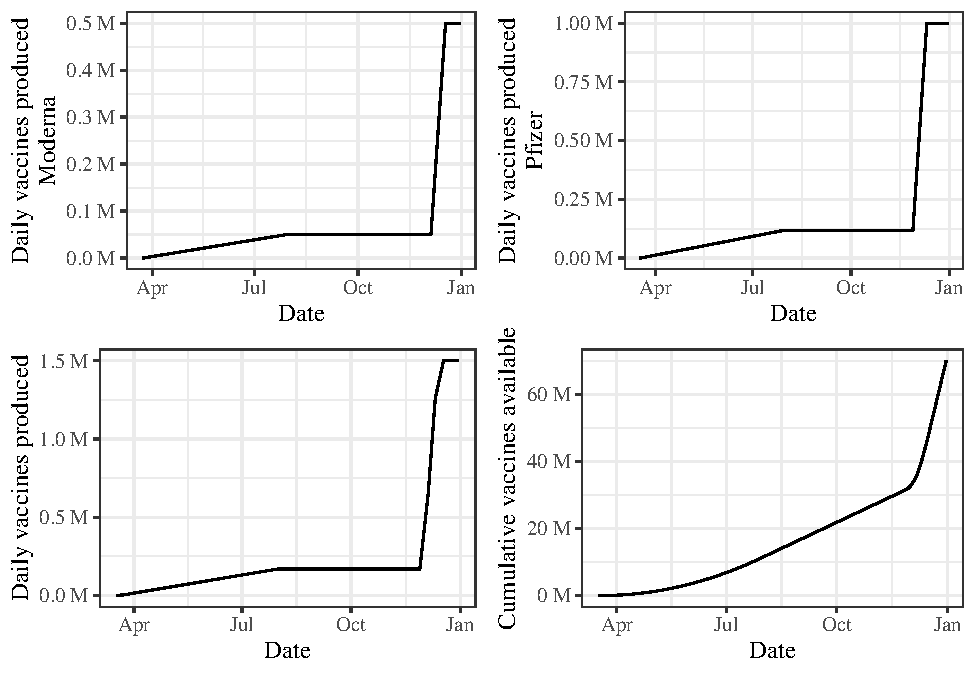
\includegraphics{_main_files/figure-latex/prod-assumptions-1} 

}

\caption{DJ9 Vaccine production assumptions}\label{fig:prod-assumptions}
\end{figure}

Figures \ref{fig:prod-cap-uk} and @rel\{fig:prod-cap-usa\} show our assumptions about the maximum number of vaccines that could be produced each day if vaccines were approved 30, 60 and 90 days earlier.

\begin{figure}

{\centering \includegraphics{_main_files/figure-latex/prod-cap-uk-1} 

}

\caption{DJ10 Limits from production UK}\label{fig:prod-cap-uk}
\end{figure}

\begin{figure}

{\centering \includegraphics{_main_files/figure-latex/prod-cap-usa-1} 

}

\caption{DJ10 Limits from production UK}\label{fig:prod-cap-usa}
\end{figure}

\bibliographystyle{apalike}



\end{document}
